\documentclass[12pt, a4paper]{article}
% Zobrazení frame - pro debug
%\usepackage{showframe}
% Tuto nechat
\usepackage{comment} 
\usepackage{lmodern}
\usepackage[inline]{enumitem}
\usepackage{xcolor}
\usepackage{blindtext}
\usepackage{scrextend}
\usepackage{cmap}
\usepackage[czech]{babel}
\usepackage[T1]{fontenc}
\usepackage[utf8]{inputenc}
\usepackage{graphicx}
\usepackage[capposition=bottom]{floatrow}
\usepackage{float}
\usepackage{amsmath}
\usepackage{hyperref}
\addtokomafont{labelinglabel}
{\sffamily}
\begin{document}

% Pouze informace
\graphicspath{ {img/} }

% Úvodní stránka
\thispagestyle{empty}
\begin{center}
\begin{minipage}{0.75\linewidth}
    \centering
%University logo
    \vspace{3cm}
    
\includegraphics[width=0.75\linewidth]{fav-logo.pdf}\\
    \vspace{0.5cm}
%Thesis title
    {\uppercase{\Large KIV/PC \\ \textbf{JednoduchÝ stemmer}\par}}
    \vspace{3cm}
%Author's name
    {\Large Jakub Vítek - A16B0165P\par}
    \vspace{2cm}
%Degree
    \vspace{1cm}
%Date
    {\Large Prosinec 2018}
\end{minipage}
\end{center}
\clearpage
\newpage

% Část obsahu dokumentu
\tableofcontents
\newpage

\section{Zadání}
\paragraph{}
\noindent Naprogramujte v ANSI C přenositelnou \textbf{konzolovou aplikaci}, která bude pracovat jako tzv. \textit{stemmer}. Stemmer je algoritmus, resp. program, který hledá kořeny slov. Stemmer pracuje ve dvou režimech: (i) v režimu \textbf{učení}, kdy je na vstupu velké množství textu (tzv. \textit{korpus}) v jednom konkrétním etnickém jazyce (libovolném) a na výstupu pak slovník (seznam) kořenů slov; nebo (ii) v režimu zpracování slov, kdy je na vstupu slovo (nebo sekvence slov) a stemmer ke každému z nich určí jeho kořen. Tento proces, tzv. \textit{stemming} je jedním ze základních stavebních kamenů nesmírně zajímavého odvětví umělé inteligence, které se označuje jako NLP (= Natural Language Processing, česky zpracování přirozeného jazyka).

\paragraph{}
Vaším úkolem je tedy implementace takového stemmeru, ovšem velice jednoduchého, podle dále uvedených instrukcí. 

\paragraph{}
Stemmer se bude spouštět příkazem \textbf{sistem.exe} (corpus-file | ["]word-sequence["]) [-msl=<\textit{celé číslo}>] [-msf=<\textit{celé číslo}>].

\paragraph{}
Symbol (\textbf{corpus-file}) zastupuje jméno vstupního textového souboru s korpusem, tj. velkým množstvím textu, který se použije k "`natrénování"'  stemmeru. Přípona souboru nemusí být uvedena; pokud uvedena není, předpokládejte, že má soubor příponu .\textbf{txt}. Symbol (\textbf{word-sequence}) zastupuje slovo nebo sekvenci slov, k nimž má stemmer určit kořeny. Režim činností programu je dán předaným parametrem. Je-li parametrem jméno (a případně cesta k) souboru, pak bude stemmer pracovat v režimu učení, tedy tvorby databáze kořenů a na základě analýzy dat z korpusu. Je-li parametrem slovo nebo sekvece slov (ta musí být uzavřena v uvozovkách), pak stemmer bude pracovat v režimu zpracování slov, tedy určování kořene každého slova ze sekvence.

\paragraph{}
Program může být spuštěn se dvěma nepovinnými parametry:

\begin{labeling}{alligator}
\item [-msl] - Nepovinný parametr \textbf{-msl=}(\textit{celé číslo}) určuje minimální délku kořene slova (msl = Minimum Stem Length), který bude uložen do databáze kořenů. Není-li tento parametr předán, použije se implicitní minimální délka kořene 3 znaky. Tento parametr je tedy zřejmě použitelný jen v kombinaci s cestou ke korpusu, teady v režimu učení stemmeru
\item [-msf] - Nepovinný parametr \textbf{-msf=}(\textit{celé číslo}) určuje minimální počet výskytů příslušného kořene (msf = Minimum Stem Frequency). Pokud se tento kořen v korpusu nevyskytl aspoň tolikrát, kolik je určeno tímto parametrem, nepoužije se při zpracování slov, tj. stemmer nemůže u žádného zpracovávaného slova oznámit, že tento kořen je kořen předmětného slova. Není-li tento parametr předán, použije se implicitní minimální počet výskytů kořene 10x. Tento parametr je tedy zřejmě použitelný jen v kombinaci se slovem nebo sekvencí slov, tedy v režimu zpracování slov.
\end{labeling}

\paragraph{}
Program může být během testování spuštěn například takto (režim učení):
\begin{verbatim}
. . . \>sistem.exe e:\data\czech-corpus.txt -msl=4
\end{verbatim}

\paragraph{}
Následně v režimu zpracování slov třeba takto:
\begin{verbatim}
. . . \>sistem.exe "šel pes do lesa" -msf=15
\end{verbatim}
\begin{verbatim}
. . . \>sistem.exe bezdomovec -msf=5
\end{verbatim}

\paragraph{}
Úkolem vašeho programu tedy je v režimu učení vytvořit databázi kořenů (textový soubor) a v režimu zpracování slov vypsat kořen každého slova ze vstupní sekvence. 

V případě, že nebude programu předán parametr prvního nebo druhého uvedeného typu, vypište krátké chybové hlášení (anglicky) a oznamte chybu operačnímu prostředí pomocí nenulového návratového kódu. Pokud bude stemmeru při prvním spuštění předáno slovo nebo sekvence slov, ukončete jej chybovým stavem (a krátkým vysvětlujícím hlášením), indikujícím, že nedošlo k předchozímu vytvoření databáze kořenů slov, a tudíž není možné u slov ze sekvence jejich kořeny určit.

\paragraph{}
Hotovou práci odevzdejte v jediném archivu typu \textbf{ZIP} prostřednictvím automatického odevzdávacího a validačního systému. Archiv nechť obsahuje všechny zdrojové soubory potřebné k přeložení programu, \textbf{makefile} pro Windows i Linux (pro překlad v Linuxu připravte soubor pojmenovaný makefile a pro Windows makefile.win) a dokumentaci ve formátu PDF vytvořenou v typografickém systému \TeX  resp. \LaTeX. Bude-li některá z částí chybět, kontrolní script Vaši práci odmítne.

\paragraph{}
Úplné zadání je dostupné na adrese:\\ \href{https://www.kiv.zcu.cz/studies/predmety/pc/doc/work/sw2018-03.pdf}{https://www.kiv.zcu.cz/studies/predmety/pc/doc/work/sw2018-03.pdf}.

% Část pro analýzu úlohy

\section{Analýza úlohy}
\paragraph{}
Stematizace (anglicky stemming) je postup, během kterého se slova převádějí na jejich základ - tzv. stem. Základem rozumíme tu část slova, která se v různých tvarech téhož slova nemění. Obvykle bývá základ slova také jeho gramatickým kořenem, nemusí tomu však být pravidlem. Často jsou příbuzná slova převedena na stejný základ, ze kterého byla odvozena a to i přes to, že daný základ nemusí být jejich gramatickým kořenem. Tyto postupy se hojně využívají při zpracování přirozeného jazyka či například jako základ pro funkcionalitu internetových vyhledavačů.

\paragraph{}
Bohužel není stematizaci možné provádět se všemi jazyky - problematická je například čínština. Většina jazyků patřících do skupiny Indo-Evropské rodiny jazyků vytváří slova na základě jasně daných gramatických pravidel. Na slova těchto jazyků je možné použít některý ze stematizačních algoritmů. Pro tyto jazyky je pak typické, že jejich základem je kořen slova, ze kterého lze odvodit slova další přidáním předpon či přípon.

\paragraph{}
Stemmer vytvářený v rámci této práce nebude pravidlový, ale statistický. Kořeny slov budou v režimu učení odvozovány analýzou velkého množství textu. Výsledkem této analýzy bude databáze všech daných kořenů spolu s počtem jejich výskytů. V režimu zpracování pak bude databáze kořenů prohledávána a ke každému detekovanému slovu ve vstupním argumentu bude třeba nalézt nejdelší kořen vyhovující nepovinnému parametru.

V rámci práce bude nutné za pomocí standardní knihovny \textit{stdio} přečíst obsah vstupního korpusu s textem. V tomto textu bude nutné nalézt slova a uložit je do některé z dostupných datových struktur. Čtení těchto dat můžeme provést načtením celé řádky a její následným rozdělením dle dělících znaků či čtením jednotlivých znaků. Načítání obsahu souboru znak po znaku je mnohem lépe kontrolované, hlavně vzhledem k tomu, že to umožnuje snáze pracovat s načítanými daty. Se znaky v tomto případě můžeme manipulovat přímo v průběhu načítání před tím, než načtený znak uložíme do vyrovnávací proměnné. Danou manipulací může být například převod velkého znaku na malý, řešení toho problému pro znaky ze sady ASCII je sice obsaženo v knihovně \textit{ctype}, ale pro znakovou sadu CP1250 potřebujeme vytvořit vlastní převodní funkci. Znaková sada CP1250 má také své vlastní dělící znaky. Manipulace při načítání nám ušetří nutnost vracet se k řetězci, jež byl načten jiným způsobem. V případě nalezení dělicího znaku pak obsah vyrovnávací paměti vložíme do zvolené datové struktury a obsah vyrovnávací paměti vynulujeme. Stejný způsob můžeme také použít při detekování slov ze vstupního argumentu. Z detekovaných slov potřebujeme vytvořit frekvenční slovní.

\paragraph{}
Po vytvoření tohoto slovníku je třeba porovnat všechna slova se všemi slovy a najít pro ně nejdelší společný podřetězec. U nalezených nejdelších společných podřetězců je následně třeba ověřit, zda jejich délka vyhovuje podmínce minimální délky. Vyhovující řetězce vkládáme do frekvenčního slovníku pro kořeny a pokud již ve vybrané datové struktuře existují, zvýšíme počitadlo výskytů slova. 

Nejvíce ideální datovou strukturou pro ukládání obou slovníku je bezpochyby trie. Spojový seznam má v nejhorším případě horší asymptotickou složitost pro detekce klíče a jeho vkládání do struktury - O(n). U hashovací tabulky bychom zase museli, pro nejvyšší efektivitu, její velikost přizpůsobit velikosti zpracovávaných dat. Při malém počtu indexů v  hashovací tabulce by nám vznikalo velké množství kolizí, jejichž řešení by při použití spojového seznamu degradovalo na asymptotickou složitost operací ve spojovém seznamu. V rámci trie nepotřebujeme řešit kolize klíčů. Také nalezení klíče má v nejhorším případě menší asymptotickou složitost - O(m), kde m reprezentuje délku klíče. Klíče vložené do trie jsou díky její struktuře logicky řazené, díky čemuž není nutné je před výpisem řadit, plně postačí průchod trií v pořadí preorder.

 
\subsection{Dostupné datové struktury}
\subsubsection{Spojový seznam}
\paragraph{}
Spojový seznam (Linked list) je strukturou určenou k ukládání dat neznámého množství. Základem spojového seznamu je uzel, který vždy obsahuje ukládanou hodnotu a ukazatel na následující prvek. Implementace vkládání dat a vyhledávání v nich je velice jednoduchá, bohužel však není příliš efektivní vzhledem k tomu, že musíme daty proiterovat v případě vkládání až na poslední prvek. V nejhorším případě se pak dostaneme na složitost O(n). Další nevýhodou je, že tato struktura ve svém základu nemá vkládané prvky abecedně či jinak řazené, prvky jsou strukturovány ve stejném pořadí, ve kterém jsou ukládány. Spojový seznam pak můžeme využít například pro implementaci hashovací tabulky. 

\begin{figure}[!ht]
	\centering
	
\includegraphics{linked-list.pdf}
	\caption{Vizualizace spojového seznamu}
\end{figure}

\subsubsection{Hashovací tabulka}
\paragraph{}
Hashovací tabulka je datovou strukturou optimalizovanou pro vyhledávání. Struktura se využívá pro ukládání dvojic klíč-hodnota. Jejím základem je standardně pole s určenou velikostí a hashovací funkce, která převádí klíče na indexy. Díky této funkci jsme schopni přistupovat na daný index se složitostí O(1), celková složitost v případě existence kolizí však záleží na implementaci úložné struktury na daném indexu - velice často je jako úložná struktura využit spojový seznam se svou složitostí O(n), alternativně je také možné pro ukládání využít binární vyhledávací strom se složitostí O(log n). Ve svém základu hashovací tabulka není seřazena. Efektivita této struktury je závislá na vhodné hashovací funkci.

\begin{figure}[H]
	\centering
	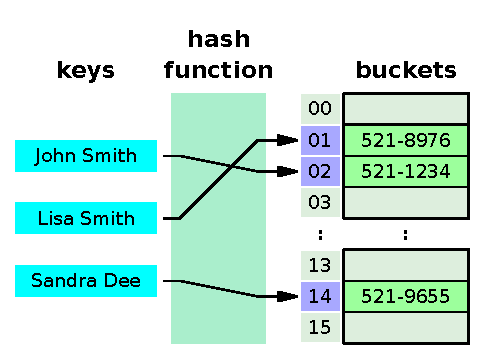
\includegraphics[scale=0.8]{hash-table.pdf}
	\caption{Vizualizace hashovací tabulky}
\end{figure}

\subsubsection{Trie}
\paragraph{}
Prefixový strom (trie) je datovou strukturou, která je používána pro ukládání dvojic klíč-hodnota, kde klíče jsou obvykle řetězci. Trie je obdobou stromu, ve kterém se podle hodnoty uzlu rozhoduje do, které větve sestoupit. V daném uzlu jsou obsaženy všechny podřetězce, kterými může pokračovat řetězec v dosud prohledané cestě. Ve standardní implementaci v rámci datové struktury nevznikají kolize klíčů. Nalezení klíče lze provést se složitostí O(m), kdy m je délka klíče. Tento způsob je mnohem rychlejší než při použití hashovací tabulky \textit{s kolizemi}. Samotná struktura svojí implementací poskytuje možnost abecedního řazení, kdy v případě, kdy chceme vypsat všechna slova vzestupně, procházíme trii v pořadí preorder. Chceme-li řadit abecedně sestupně, procházíme trii v pořadí postorder. Často se Trie využívá pro implementaci slovníků.  

\begin{figure}[H]
	\centering
	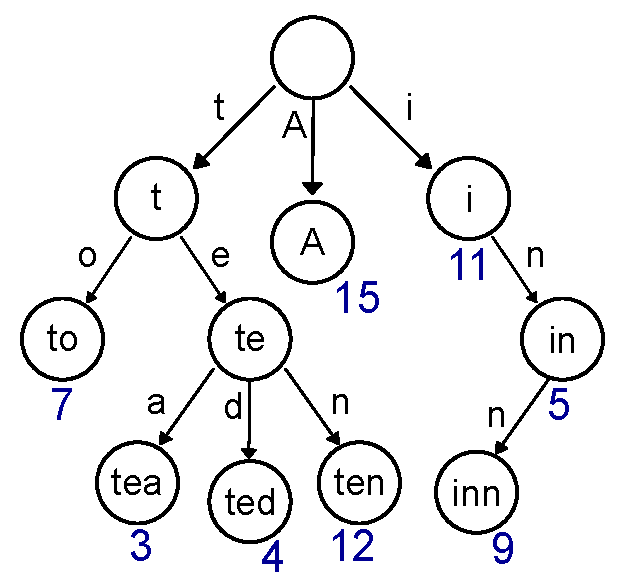
\includegraphics[scale=0.6]{trie.pdf}
	\caption{Vizualizace datové struktury Trie}
\end{figure}

% Část pro popis implementace
\newpage
\section{Popis implementace}
\subsection{Datové struktury a typy}
\subsubsection{Struktura aplikačního kontextu}
\paragraph{}
Struktura \textit{app\_context} je základem pro řízení aplikace. Pro její vytvoření předáváme pole argumentů programu z příkazové řádky spolu s jejich počtem. Tato data jsou dále zpracována, například je zde určeno, zda je vstupem název souboru, cesta k němu či se jedná o slovo či jeho sekvenci. V rámci tvorby této struktury jsou také parsovány nepovinné vstupy programu. V případě jakékoliv chyby funkce vytvářející tuto strukturu vrátí ukazatel NULL. Tato struktura je velice důležitá pro chod aplikace, na základě informací uložených uvnitř této struktury řízena zbylá část programu. 

\subsubsection{Struktura jednoho prvku spojového seznamu}
\paragraph{}
Struktura \textit{list\_node} je standardní implementací jednoho prvku spojového seznamu. Uvnitř této struktury je obsažen ukazatel na počátek řetězce, který má být v rámci daného prvku ukládán spolu s číselnou hodnotou, která reprezentuje počet výskytů ukládaného řetězce. Nakonec je obsahem struktury také ukazatel na další prvek spojového seznamu, tento ukazatel je pak možné opakovaně využívat pro iteraci prvků spojového seznamu.

\subsubsection{Struktura jednoho uzlu trie}
\paragraph{}
Struktura \textit{trie\_node} představuje jeden z uzlů datové struktury trie. Struktura obsahuje dvě číselné proměnné, jednou z nich je příznak, zda aktuální uzel je koncem slova a druhou pak počet výskytů slova (či prefixů, nejedná-li se o konec slova). Součástí struktury je také pole o velikosti zpracovávané abecedy znaků, v případě této práce se jedná o 255 ukazatelů na další uzel, z nichž všechny jsou nejprve nastaveny na NULL. Tyto ukazatele jsou inicializovány v případě potřeby, například, chceme-li od kořenového uzlu vkládat znak "`a"' (ASCII hodnota 97), vytvoříme strukturu \textit{trie\_node} a ukazatel na ni uložíme do pole ukazatelů v kořenovém uzlu na index 97.


% Část pro moduly
\subsection{Popis modulů}
\subsubsection{Modul main.c}
\paragraph{}
Tento modul slouží jako vstupní bod aplikace. 

\paragraph{}
Funkce \textit{int main(int argc, char *argv[]} je volána při spuštění aplikace. Funkce při svém běhu vytváří strukturu \textit{app\_context} voláním funkce \textit{create\_app\_context} a předáním argumentů \textit{argc} a \textit{argv}. Následně je ověřována validita této struktury ověřováním jejího obsahu, při chybě je program ukončen s návrácením chybového kódu (s případně předcházející zprávou o chybě). Není-li ukazatel na \textit{app\_context} NULL, ověřuje se také proměnná struktury \textit{error\_code}, která při nenulové číselné hodnotě indikuje chybu při zpracování vstupu. Při úspěšné validaci se na základě dat uložených ve struktuře rozhoduje o spuštění modulů \textit{learning\_mode} pokud pole argumentů programu obsahovalo název souboru či cestu k němu. Modul \textit{processing\_mode} je pak spušten v případě, kdy je na vstupu detováno slovo či sekvence slov, přičemž detekce je prováděna pokusem o otevření souboru za použití vstupního argumentu jako názvu testovaného souboru. Lze-li soubor přečíst, bude provedeno spuštění modulu \textit{learning\_mode}, v opačném případě pak spuštění modulu \textit{processing\_mode}.  
 
\subsubsection{Modul learning\_mode.c}
\paragraph{}
Modul, jež provádí vytváření slovníku kořenů. 

\paragraph{}
Funkce \textit{int learning\_mode(app\_context *context)} po svém zavolání nejprve ověřuje validitu vstupu. V případě zjištění jakýchkoliv chyb jsou všechny využívané zdroje uvolňěny a je navrácen příslušný návratový kód, díky kterému lze rozpoznat typ chyby. V případě, že je vstup validní, je vytvořen kořenový prvek \textit{trie} a následně provedena detekce slov při čtení souboru. Název či cesta k souboru jsou uloženy uvnitř aplikačního kontextu. Soubor je čten znak po znaku a ukládán do vyrovnávací proměnné do té doby, než načtený znak je jedním z definovaných rozdělovačů slov, v tomto případě se na konec doposud načteného řetězce vloží ukončovací znak řetězce. Detekované slovo je pak  vloženo do \textit{trie} a vyrovnavací paměť vynulována. Postup je následně opakován do nalezení konce souboru. Načteme-li znak vyjadřující velké písmeno, převádíme jej před vložením do vyrovnavací paměti na písmeno malé.

Pro všechna nazená slova vytvoříme jejich kombinace tak, že pro každé iterované slovo vytvoříme kombinaci s každým iterovaným slovem, ve výsledku tak získáváme $n^2$ kombinací. Na tyto kombinace pak aplikujeme funkci \textit{longest\_common\_substring}, kombinace však neprocházíme všechny. V případě, že zde máme kombinaci například \textit{ahoj} a \textit{jablko}, výsledek nejdelšího společného podřetězce bude stejný jako pro kombinaci \textit{jablko} a \textit{ahoj}. Výsledek funkce \textit{longest\_common\_substring} vkládáme do \textit{trie}, která reprezentuje slovník nalezených kořenů. Všechny nalezené kořeny spolu s počtem jejich výskytů využitím funkce \textit{trie\_to\_file} vypíšeme v požadovaném formátu do souboru \textit{stems.dat}. Jsou-li všechny operace v modulu úspěšné, je navrácen kód \textit{0}.

\subsubsection{Modul processing\_mode.c}
\paragraph{}
V tomto modulu je čten vytvořený slovník kořenů do datové struktury. Ze vstupního řetězce v aplikačním kontextu je vytvořen spojový seznam slov, který je iterován. Pro každé nalezené slovo tak hledáme jeho kořen. 

\paragraph{}
Funkce \textit{int processing\_mode(app\_context *context)} po svém zavolání nejprve ověřuje, zda předaný aplikační kontext a jeho data existují a jsou v požadovaném tvaru, případě neúspěchu tohoto uvolnění jsou všechny zdroje alokované v rámci této funkce uvolněny. Po úspěšném ověření je za pomocí funkce \textit{file\_read\_database\_to\_trie} načten frekvenční slovník ze souboru \textit{stems.dat} do trie. Při ukládání do trie jsou ignorovány všechny kořeny, které nevyhovují nepovinnému parametru minimálního výskytu kořenů.
 
Po prečtení frekvenčního slovníku do trie je provedena detekce slov ze vstupního argumentu za využití funkce \textit{string\_read\_words\_to\_list}, nalezená slova jsou uložena do spojového seznamu. Následně je tento seznam iterován a pro každé slovo hledáme jeho kořen voláním funkce \textit{trie\_find\_longest\_stem}. V případě nalezení kořene jej vypíšeme, v opačném případě k danému vstupnímu slovu vypíšeme \textit{0}. Před navrácením kódu úspěchu vždy uvolňujeme veškeré alokované zdroje.

\subsubsection{Modul context.c}
\paragraph{}
Modul pro tvorbu aplikačního kontextu. V rámci tohoto modulu jsou zpracovány veškeré vstupy z příkazové řádky a uloženy do struktury \textit{app\_context}.

\paragraph{}
Funkce \textit{app\_context *create\_app\_context(int argc, char **argv)} vrací odkaz na strukturu \textit{app\_context}. Jako vstup předpokládá argumenty z příkazové řádky spolu s jejich počtem, nedostane-li minimální počet argumentů, vnitřní proměnná struktury \textit{error\_code} je nastavena na nenulové číslo indikující chybu při zpracování argumentů programu. V tomto případě je navrácen ukazatel na strukturu, jež obsahuje tento indikátor chyby. 
V případě, že počet vstupních argumentů vyhovuje minimálnímu počtu, je u prvního argumentu detekováno, zda se jedná o název souboru (či cestu k němu) nebo slovo (či sekvenci slov). Detekce je prováděna pokusem o otevření souboru ke čtení s tímto textem. Podařila-li se tato operace, do struktury je vstupní argument uložen jako název (cesta k) souboru. V opačném případě je vstupní argument uložen jako slovo (či sekvence slov). 
V poslední případě funkce zpracovává nepovinné parametry. Toho je docíleno tím, že je nejprve určen parametr detekcí prefixu řetězce (například řetězec -msl=2 má prefix -msl=). Tento prefix je dále zanedbán a zpracuje se pouze zbytek řetezce následující po daném prefixu funkcí \textit{strtol} pro převedení na číselnou hodnotu. Po provedení funkce strtol ještě za pomocí technik aritmetiky ukazatelů a hodnoty errno ve funkci \textit{strtol\_error\_detect} detekuje chyba při převedení řetezce na číslo. Nastane-li při převodu chyba, proměnná struktury app\_context \textit{error\_code} bude nastavena na příslušný chybový kód.

\paragraph{}
Funkce \textit{int file\_exists(const char *file\_name)} vrací \textit{nulovou hodnotu} v případě, že vstupní řetězec není názvem souboru či cestou k němu. Detekce je prováděna pokusem o otevření souboru ke čtení. V případě, že může být soubor přečten, je navrácena hodnota \textit{1}.

\paragraph{}
Funkce \textit{int string\_starts\_with(const char *prefix, const char *string)} detekuje zda je vstupní řetězec \textit{prefix} prefixem vstupního řetězce \textit{string}. Detekce je provedena voláním funkce \textit{strncpy}, která porovná prefix s řetězcem string zkráceným na délku řetězce prefix. Vrací nulovou hodnotu v případě, že řetězec prefix není prefixem řetezce string, v opačném případě vrátí číslo 1.

\paragraph{}
Funkce \textit{void free\_app\_context(app\_context *context)} uvolní pamět alokovanou pro strukturu \textit{app\_context}. Nejprve je uvolněna pamět pro vnitřní proměnné struktury, teprve pak je uvolněna struktura jako taková.
  
\paragraph{}
Funkce \textit{int strtol\_error\_detect(char *nptr, char **endptr, long number)} na základě hodnoty errno nastavené při přecházejícím převodu řetězce na číslo a ukazatele \textit{endptr} detekuje chybu. V případě detekce chyby je vrácena hodnota \textit{1}, v opačném případě hodnota \textit{0}.

\subsubsection{Modul linked\_list.c}
Modul, který obsahuje všechny potřebné definice a funkce pro práci se spojovým seznamem ukládajícím řetězec a počet jeho výskytů.

\paragraph{}
Funkce \textit{list\_node *create\_list\_node(char *string, int count)} vytváří strukturu \textit{list\_node} reprezentující jeden z uzlů spojového seznamu. Funkce validuje vstupy, v případě, že ukazatel na řetězec string je NULL či je zadán nevalidní počet výskytů není uzel vytvářen a je navrácen ukazatel NULL. V případě validních dat jsou oba vstupy uloženy do struktury.

\paragraph{}
Funkce \textit{void insert\_list\_string(list\_node *root,char *string, int count)} nejprve vytváří ze vstupního řetězce \textit{string} a čísla \textit{count} uzel spojového seznamu a následně volá funkci \textit{insert\_list\_node} pro vložení uzlu do spojového seznamu.

\paragraph{}
Funkce \textit{void insert\_list\_node(list\_node *root, list\_node *item)} vkládá vytvořený uzel spojového seznamu na konec spojového seznamu. Konec seznamu je detekován opakovaným procházením ukazatele \textit{next} v jednotlivých strukturách \textit{list\_node}.

\paragraph{}
Funkce \textit{void print\_list(list\_node *root)} prochází spojový seznam za pomocí odkazu \textit{next} ve struktuře \textit{list\_node}. 

\paragraph{}
Funkce \textit{void free\_list(list\_node *root)} uvolní pamět alokovanou pro všechny uzly spojového seznamu s počátkem v uzlu \textit{root}. Při uvolňování paměti je seznam iterován, vždy je nejprve uložen ukazatel na aktuálně iterovaný prvek do dočasné proměnné, následně je ukazatel aktuálně iterovaného prvku nastaven na prvek v iteraci následující. Následně je alokovaná paměť uvolněna pomocí ukazatelé v dočasné proměnné. Iterace je prováděna do doby, než následující prvek iterace je NULL.


\subsubsection{Modul trie.c}
\paragraph{}
Tento modul obsahuje všechny potřebné funkce a definice pro práci s trií, jež ukládá řetězce a počet jejich výskytů.

\paragraph{}
Funkce \textit{trie\_node *create\_trie\_node()} vytvoří nový uzel pro Trii. Tato struktura (\textit{trie\_node}) obsahuje počítadlo výskytů a proměnnou indikující, zda se jedná o konec slova. Dále je uvnitř struktury pole ukazatelů na následující uzly \textit{trie\_node} ve velikosti abededy - v našem případě 255 položek při vytváření nastavených na NULL.

\paragraph{}
Funkce \textit{void trie\_insert(trie\_node *root, char *key)} vkládá do trie, jejíž kořenovým uzlem je vstup \textit{root}. Vkládání řetězce je prováděno po jeho jednotlivých znacích. Vkládáním znaků je vytvářen strom, pokud znak na vkládané pozici již má svůj uzel, je pouze zvýšeno počítadlo výskytů, v opačném případě je v dané cestě strome vytvořen nový uzel.

\paragraph{}
Funkce \textit{int trie\_is\_leaf\_node(trie\_node *node)} zjišťuje zda v uzlu určeném vstupem \textit{node} končí slovo. Vrací 1 v případě, že uzel je koncem slova, v opačném přípravě vrátí hodnotu 0.

\paragraph{}
Funkce \textit{void trie\_free(trie\_node *root)} uvolňuje pamět alokovanou aktuálním uzlem v trii a všemi uzly v trii následujícími. Funkce je rekurznivní, nejprve jsou vždy uvolňovány následující uzly, teprve následně uzel aktuální. 

\paragraph{}
Rekurzivní funkce \textit{void trie\_display(trie\_node *root, char *str, int level)} zajištuje výpis všech klíčů uložených do trie. Vstup \textit{str} určuje aktuálně načtený řetězec a vstup \textit{level} určuje hloubku uzlu v trii. Klíč je vypsán v případě, kdy je při průchodu nalezen nenulový příznak konce slova. 

\paragraph{}
Funkce \textit{void trie\_to\_list(list\_node *list\_root,trie\_node *root, char *str, int level)} funguje podobným způsobem jako funkce \textit{trie\_display} s tím rozdílem, že jsou nalezená slova místo výpisu na standardní výstup ukládána do spojového seznamu.

\paragraph{}
Funkce \textit{void trie\_to\_file(FILE *file, trie\_node *root, char *str, int level)} funguje podobným způsobem jako funkce \textit{trie\_display} a \textit{trie\_to\_list} s tím rozdílem, že je výstup formátován a ukládán do textového souboru.

\paragraph{}
Funkce \textit{void trie\_find\_longest\_stem(trie\_node *node, char *word, char *buffer, int level, char *output)} rekurzivně prochází uzly trie v podobně jako například u funkce \textit{trie\_display}. V případě nalezení klíče pak zjistí, zda má klíč (\textit{obsah vstupu buffer}) a hledané slovo (\textit{word}) společný podřetězec. V případě, že takový podřetězec existuje, zjištuje se, zda aktuálně nalezený klíč (kořen) je delší než doposud nejdelší nalezený kořen (v ukazateli \textit{output}).

\subsubsection{Modul string\_helper.c}
\paragraph{}
Tento modul obsahuje různé pomocné funkce pro manipulaci se znaky, rětězci či jejich délkami.

\paragraph{}
Funkce \textit{int cp1250\_is\_word\_separator(unsigned char c)} určuje zda vstupní znak \textit{c} je oddělovačem slov v kodovani CP1250. Funkce obsahuje pole se všemi dělícími znaky, funkce tak zjištuje zda daný znak je součástí tohoto pole. V případě, že je vstupní znak znakem dělícím slova, funkce vrací hodnotu 1, v opačném případě je vrácena hodnota 0. 

\paragraph{}
Funkce \textit{unsigned char cp1250\_tolower(unsigned char c)} vrací hodnotu znaku převedeného na malé písmeno pro kódování CP1250. Pro převod znaku v rozsahu kódování ASCII (0 až 127) je využita funkce \textit{tolower}.

\paragraph{}
Funkce \textit{long long\_max(long a, long b)} vrací větší číslo ze dvou vstupů \textit{a} a \textit{b}.
 

\subsubsection{Modul file\_helper.c}
\paragraph{}
Modul, který obsahuje různé pomocné funkce pro uložení dat do různých datových struktur.

\paragraph{}
Funkce \textit{int string\_read\_words\_to\_list(char *string, list\_node *node)} ve vstupním řetězci \textit{string} detekuje slova a ukládá je do spojového seznamu. Detekce slov je prováděna funkcí \textit{strtok}, které je předáno pole s oddělovacími znaky. Iterace mezi jednotlivými slovy nalezenými funkcí strtok je provedena opakovaným voláním funkce s prvním parametrem rovným NULL. 

\paragraph{}
Funkce \textit{int file\_read\_database\_to\_trie(char *file\_name, trie\_node *root, long msf)}, která je určena pro přečtení souboru \textit{stems.dat}. Funkce také provádí detekci kořenů a frekvencí jejich výskytu použitím funkce \textit{fscanf}. Pro každý nalezený kořen a jeho frekvenci je pak ověřováno, zda množství kořenů vyhovuje nepovinnému parametru \textit{minimum stem frequency}. V případě, že množství kořenů nevyhovuje minimální frekvenci, není daný kořen uložen do trie. 

\subsubsection{Modul lcs.c}
\paragraph{}
Tento modul kompletní řešení pro nalezení nejdelšího společného podřetězce dvou řetězců.

\paragraph{}
Funkce \textit{unsigned int longest\_common\_substring(char *str1, char *str2, char **result)} ke vstupům \textit{str1} a \textit{str2} hledá nejdelší společný podřetězec těchto vstupní řetězců a ukládá jej na adresu určenou vstupem \textit{result}. Vnitřně si funkce vytváří dvourozměrné pole (matice) o velikosti $(i + 1) x (j + 1)$, kde \textit{i} je délkou řetězce \textit{str1} a \textit{j} je pak délkou řetězce \textit{str2}. První řádek a první sloupec matice bude obsahovat nulu vzhledem k tomu, že jakýkoliv rětězec spolu s prázdným rětězcem mají délku největšího společného podřetězce nulovou. Zbylé části matice jsou vyplňovány dle výsledku následující funkce:

\[ LCS(X_{i..n}, Y_{j..m}) =
    \begin{cases}
        LCS(X_{i..n - 1}, Y_{j..m - 1})		& \quad \text{pokud } X[i] = Y[j] \\
        0 									& \quad \text{jinak}
    \end{cases}
\]

Algoritmus následně postupuje u nenulových čísel po diagonále, nejdelší nenulová sekvence čísel diagonálách z levé horní část do pravé dolní části pak určuje nejdelší společný podřetězec.

% Část pro uživatelskou dokumentaci
\newpage
\section{Uživatelská příručka}
\subsection{Podporované operační systémy}
\paragraph{}
Aplikaci je možné sestavit pro operační systémy Microsoft Windows, GNU/Linux a Mac OS v případě, že jsou na vybraném operačním systému nainstalovány nástroje \textit{gcc} a \textit{make}.

\paragraph{}
V operačním systému GNU/Linux lze tyto nástroje získat jejich instalací z repozitáře, které se liší pro každou distribuci.

\paragraph{}
Pro operační systém Microsoft Windows je doporučováno využít nástrojů MinGW, Cygwin pro získání těchto nástrojů.

\subsection{Spuštění programu}
\paragraph{}
Program lze spusti ve dvou režimech, v režimu učení a v režimu zpracovávání. Nejprve je nutné spustit program v režimu učení a jako vstup mu předat název (či cestu k) souboru. Toto je nutné pro prvotní vytvoření frekvenčního slovníku kořenu, ukládaného do souboru \textit{stems.dat}. Program v režimu učení lze spustit následovně: 

\begin{verbatim}
. . . \>sistem.exe e:\data\czech-corpus.txt
\end{verbatim}

\paragraph{}
Po vytvoření frekvenčního slovníku kořenů lze program spustit v režimu zpracovávání. V tomto případě je nutné programu předat ve vstupním argumentu slovo či sekvenci slov. Program v režimu učení lze spustit následujícím způsobem:

\begin{verbatim}
. . . \>sistem.exe "šel pes do lesa a potkal dlažební kostku"
\end{verbatim} 

V případě jediného slova můžu spuštění vypadat následovně:

\begin{verbatim}
. . . \>sistem.exe pes -msl=4
\end{verbatim}

\paragraph{}
Program také reaguje na nepovinné parametry \textit{-msl} a \textit{-msf}, které oba zpracovává v obou režimech programu.  

% Část pro shrnutí a konec 
% TODO: závěr, 
\newpage
\section{Závěr}
\subsection{Časy běhu programu}
Časy běhu programu v obou režimech byly prováděny na stolním počítači vlastního sestavení s konfigurací Intel Core i5-6500, 16GB paměti RAM a SSD Samsung SSD 850 EVO 250GB.

\paragraph{}
V režimu učení program dosahoval následující časů:
\begin{center}
 \begin{tabular}{||l  |  c  ||}  
 \hline
 Spuštěný příkaz & Čas běhu  \\ [0.5ex] 
 \hline\hline
 ./sistem.exe dasenka.txt & 1.964 sec \\ 
 \hline
 ./sistem.exe dasenka.txt -msl=4 & 1.744sec \\ 
 \hline
 ./sistem.exe kultura.txt & 428.156 sec \\ [1ex] 
 \hline
\end{tabular}
\end{center}

\paragraph{}
V režimu zpracování program dosahoval následujících časů (pro stems.dat vytvořený v režimu učení ze souboru dasenka.txt):

\begin{center}
 \begin{tabular}{||l | c  ||} 
 \hline
 Spuštěný příkaz & Čas běhu  \\
 \hline\hline
 ./sistem.exe pes & 0.008 sec \\ 
 \hline
 ./sistem.exe "šel pes do lesa a potkal dlažební kostku" -msl=4 & 0.014sec \\ 
 \hline
 ./sistem.exe [lorem ipsum 200 slov] & 0.144 sec \\ 
 \hline
\end{tabular}
\end{center}

\subsection{Shrnutí}
\paragraph{}
S jazykem C příliš často nepracuji, při zpracování programu jsem měl velice krušné začátky, kdy jsem si potřeboval osvěžit všechny vlastnosti a zákonitosti jazyka C. Velkým problémem pro mě byl nástroj valgrind, jež jsem nakonec byl schopný využít pro správu paměti bez tzv. memory leaků. Čím déle jsem na projektu pracoval, tím snáze jsem řešil veškeré problémy, které při vývoji nastaly.

\subsection{Zhodnocení práce}
\paragraph{}
Program splňuje zadání semestrální práce, bohužel však využívá o mnoho více paměti RAM, než bylo původním předpokladem (300MB až 500MB). Využití paměti je závislé na velikosti vstupního souboru.

Pro malé vstupní korpusy je program rychlý, doba jeho běhu narůstá s jejich velikostmi. Program je relativně rychlý, existuje zde však prostor pro optimalizaci, hlavně co se algoritmu LCS a využití paměti týče.


\newpage
\listoffigures



\end{document}